\section{STL Generation and Mesh Processing}

\subsection{STL Generation Using Gmsh}

After the parameterized geometry has been defined using Gmsh, the next step is to export the geometry into a more suitable format for further processing. This is done by exporting the geometry as an STL (stereolithography) file, which represents the surface of the geometry as a collection of triangles. Gmsh provides built-in functionality to export geometries in STL format, ensuring that the generated mesh can be easily processed by other tools.

During the STL generation, important settings such as mesh refinement are specified to ensure that the final geometry captures all the necessary details. Mesh refinement controls the density of triangles on the surface, and it's crucial to balance the level of detail with computational efficiency. A finer mesh may result in better simulation accuracy but increases the computational cost.

\subsection{Processing the STL with Trimesh}

Once the STL file is generated, it is loaded into the Python environment using the Trimesh library, which offers powerful tools for manipulating 3D meshes. Trimesh allows the conversion of the STL surface mesh into a rectilinear (voxel) mesh, a format better suited for numerical simulations such as the Lattice Boltzmann Method (LBM).

The conversion process involves discretizing the surface of the geometry into a grid of voxels, where each voxel represents a cubic element of the mesh. This voxelization ensures that the mesh can be used in simulations that require structured grids, such as fluid dynamics simulations. Trimesh provides various utilities for handling this conversion, and the resulting voxel mesh is stored as a 3D NumPy array for further use.

% [Figure suggestion: A comparison of the original STL mesh and the voxelized mesh, highlighting the transformation from surface to voxel representation.]

\begin{figure}[H]
	\centering
	\vspace{6mm}
	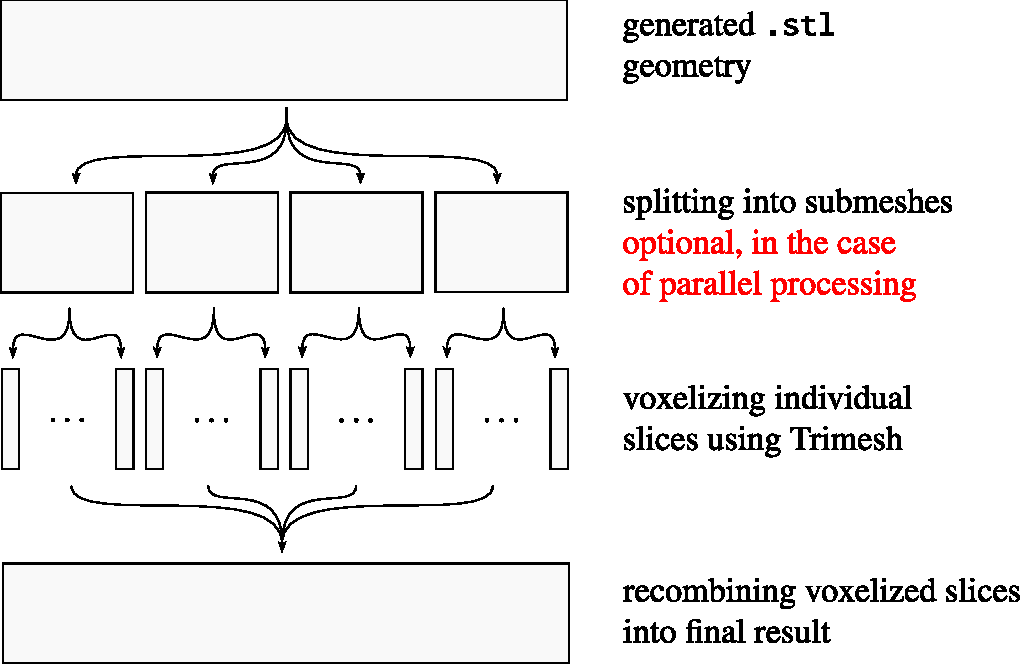
\includegraphics[width=.77\textwidth]{figures/voxelizing.pdf}
	\vspace{4mm}
	\caption{Overview of the \texttt{meshgen} package.}
	\label{fig:voxelizing}
\end{figure}